\documentclass[10pt,landscape]{article}
\usepackage{multicol}
\usepackage{calc}
\usepackage{amsmath,amsthm,amsfonts,amssymb,relsize}
\usepackage{color,graphicx,overpic}
\usepackage{enumitem}
\usepackage{bm}
\usepackage[cheatsheet]{preamble}
\definecolor{MyRoyalBlue}{RGB}{65,105,225} % RGB for Royal Blue
\definecolor{SubsectionGreen}{RGB}{180, 175, 80} % A soft green
% Turn off header and footer
\pagestyle{empty}
\geometry{top=.25in,left=.25in,right=.25in,bottom=.25in}


\definecolor{MyRoyalBlue}{RGB}{65,105,225} % RGB for Royal Blue
\definecolor{SubsectionGreen}{RGB}{75, 175, 80} % A soft green

% Redefine section commands to use less space
\makeatletter
\renewcommand{\section}{\@startsection{section}{1}{\z@}{3ex}{2ex}
                       {\normalfont\normalsize\bfseries\color{MyRoyalBlue}\textit}}
\renewcommand{\subsection}{\@startsection{subsection}{2}{\z@}{2ex}{0.5ex}
                          {\normalfont\small\bfseries\color{SubsectionGreen}}}
\renewcommand{\subsubsection}{\@startsection{subsubsection}{3}{0mm}%
                          {-1ex plus -.5ex minus -.2ex}%
                          {1ex plus .2ex}%
                          {\normalfont\small\bfseries}}
\makeatother

\setlist[itemize]{label={}, leftmargin=*, topsep=0pt, parsep=0.5pt, partopsep=0pt} % Remove margins from lists. 

% Don't print section numbers
\setcounter{secnumdepth}{0}

\setlength{\parindent}{0pt}
\setlength{\parskip}{0pt}

\newcommand{\R}{\mathbb{R}}
\newcommand{\E}{\mathbb{E}}

\newcommand{\bb}{\mathbf{b}}
\newcommand{\bv}{\mathbf{v}}
\newcommand{\bx}{\mathbf{x}}
\newcommand{\by}{\mathbf{y}}
\newcommand{\bz}{\mathbf{z}}

\newcommand{\bA}{\mathbf{A}}
\newcommand{\bB}{\mathbf{B}}
\newcommand{\bH}{\mathbf{H}}
\newcommand{\bI}{\mathbf{I}}
\newcommand{\bJ}{\mathbf{J}}
\newcommand{\bX}{\mathbf{X}}
\newcommand{\bY}{\mathbf{Y}}
\newcommand{\bZ}{\mathbf{Z}}

\newcommand{\balpha}{\boldsymbol{\alpha}}
\newcommand{\bbeta}{\boldsymbol{\beta}}
\newcommand{\btheta}{\boldsymbol{\theta}}
\newcommand{\bmu}{\boldsymbol{\mu}}
\newcommand{\bxi}{\boldsymbol{\xi}}
\newcommand{\bSigma}{\boldsymbol{\Sigma}}
\newcommand{\bLambda}{\boldsymbol{\Lambda}}

\newcommand{\diag}{\text{diag}}
\newcommand{\tp}[1]{#1^{\prime}}
\newcommand{\inv}[1]{#1^{-1}}
\newcommand{\norm}[1]{\|#1\|}
\newcommand{\gaussian}[2]{\mathcal{N}(#1, #2)}
\newcommand{\inR}[2]{#1 \in \R^{#2}}


\newcommand{\ruler}{\\\rule{\linewidth}{0.25pt}\\}

% -----------------------------------------------------------------------
\begin{document}
\raggedright%
\footnotesize
\begin{multicols*}{3}
    % multicol parameters
    % These lengths are set only within the two main columns
    % \setlength{\columnseprule}{0.1pt}
    \setlength{\premulticols}{1pt}
    \setlength{\postmulticols}{1pt}
    \setlength{\multicolsep}{1pt}
    \setlength{\columnsep}{0pt}

    \section{Math Review}
    \begin{itemize}
        \item $\bX$ and $\bY$ are \textbf{independent} iff $P(\bX,\bY)=P(\bX)P(\bY)$
        \item $\bX$ and $\bY$ are \textbf{uncorrelated} iff $\E(\bX,\bY)=\E(\bX)\E(\bY)$
        \item \underline{Expected} value of $g(X)$ : \( E[g(X)] = \int_{-\infty}^{\infty}g(x)f(x) dx\)
        \item \underline{Variance} \( \sigma^2 = E[(X - \mu)^2] = E[X^2] - \mu^2\)
        \item Determinant of matrix is product of its eigenvalues.
    \end{itemize}
    $
        f(\bx) = \bA\bx + \tp{\bx}\bA + \tp{\bx}\bx + \tp{\bx}\bA\bx \Rightarrow
        \frac{df(\bx)}{d\bx} = \tp{\bA} + \bA + 2\bx + \bA\bx + \tp{\bA}\bx
    $
    \begin{align*}
        \nabla_{\bm{x}} (\bm{y} \cdot \bm{z}) & = (\nabla_{\bm{x}}) \bm{z} + (\nabla_{\bm{x}}) \bm{y} & \nabla_{\bm{x}} f(\bm{y}) & = (\nabla_{\bm{x}} \bm{y}) (\nabla_{\bm{y}} f(\bm{y})) \\
        \nabla_w w^TAw                        & = (A + A^T)w                                          & \bH_{i,j}                 & = \frac{\partial^2 f}{\partial x_i \partial x_j}
    \end{align*}
    \section{Perceptron (Lecture 2)}
    $f(\bx) = \mathbf{w} \cdot \bx + \alpha = \sum_{i=1}^{d}w_ix_i + \alpha$,


    \textbf{Goal: } find $w$ s.t all constraints $y_i X_i \cdot w \ge 0$. Define a risk function and optimize it, where the loss is defined as $L(z, y_i) = -y_iz \;\text{  if } y_iz < 0, \;\text{else }0$. Therefore risk $R(w) = \sum_{i \in V}-y_i X_i \cdot w$
    \ruler
    \textbf{Decision boundary}, a \textbf{hyperplane} in $\R^d$: $H = \{\inR{\bx}{d} : f(\bx) = 0\} = \{\inR{\bx}{d} : \mathbf{w} \cdot \bx + \alpha = 0\}$
    \ruler
    $\mathbf{w}$ is the \textbf{normal} of the hyperplane,\\
    $\alpha$ is the \textbf{offset} of the hyperplane from origin,\\
    $\frac{f(\bx)}{\norm{\mathbf{w}}}$ is the \textbf{signed distance} from the \( \bx \) to hyperplane \( \mathcal{H} \).
    \ruler
    \textbf{Perceptron algorithm},\\
    Input: $(\bx_1, y_1),\dots,(\bx_n, y_n) \in \R^{d} \times \{\pm 1\}$\\
    while some $y_i \neq \text{sign}(\mathbf{w} \cdot \bx_i)$\\
    \-\hspace{0.5cm} pick some misclassified $(\bx_i, y_i)$\\
    \-\hspace{0.5cm} $\mathbf{w} \leftarrow \mathbf{w} + y_i\bx_i$
    \ruler
    Given a \textbf{linearly separable data}, perceptron algorithm will take no more than $\frac{R^2}{\gamma^2}$ updates to \textbf{converge},
    where $R = \max_{i}{\norm{\bx_i}}$ is the radius of the data, $\gamma = \min_{i}{\frac{y_i(\mathbf{w}\cdot\bx_i)}{\norm{\mathbf{w}}}}$ is the margin.\\
    Also, $\frac{\mathbf{w}\cdot\bx}{\norm{\mathbf{w}}}$ is the signed distance from H to $\bx$ in the direction $\mathbf{w}$.
    \ruler
    \textbf{Gradient descent} view of perceptron, minimize margin cost function
    $J(\mathbf{w}) = \sum_{i}(-y_i(\mathbf{w}\cdot\bx_i))_{+}$ with $\mathbf{w} \leftarrow \mathbf{w} - \eta\nabla J(\mathbf{w})$
    % --------------------------------

    \section{Support Vector Machine (Lecture 3, 4)}
    \textbf{Hard margin SVM},\\
    This method makes the margin as wide as possible.
    The signed distance from the hyperplane to $X_i$ is$\frac{f(\bx_i)}{\lVert w \rVert}$
    Hence the margin is $\min_i \frac{1}{\lVert w \rVert} |w \cdot X_i + \alpha|  \ge \frac{1}{\lVert w \rVert} \implies$
    $\min_{\mathbf{w}} \norm{\mathbf{w}}^2$, such that $y_i\mathbf{w}\cdot\bx_i \geq 1 (i = 1,\dots,n)$\\
    \textbf{Soft margin SVM},\\
    $\min_{\mathbf{w}} \norm{\mathbf{w}}^2 + C\sum_{i = 1}^{n} \xi_i$
    \ruler
    \textbf{Regularization and SVMs}:
    Simulated data with many features $\phi(\bx)$;
    C controls trade-off between margin $1/\norm{\mathbf{w}}$ and fit to data;
    Large C: focus on fit to data (small margin is ok). More overfitting.
    Small C: focus on large margin, less tendency to overfit.
    Overfitting increases with: less data, more features.
    % --------------------------------
    \section{Decision Theory (Lecture 6)}
    \textbf{Bayes Theorem:} \( \underbrace{P(Y = C | X)}_{\text{Poster. Prob}} = \frac{P(X | Y = C) \overbrace{P(Y = C)}^{\text{Prior Prob.}}}{P(X)} \)
    Assume $(\bX, \bY)$ are chosen i.i.d according to some probability distribution on $\mathcal{X}\times\mathcal{Y}$.
    \textbf{Risk} is misclassification probability: $R(r) = \E (L(r(\bX), \bY)) = Pr(r(\bX)
        \neq \bY) =$

    \( \sum_\bx \big[ L(r(\bx), 1)P(Y = 1|x) + L(r(x), -1)P(Y = -1|X = \bx) \big] \times P(\bx \)
    \ruler
    \( = P(Y = 1) \sum_x L(r(\bx), 1)P(\bx|Y = 1) + P(Y = -1) \sum_x L(r(\bx), -1)P(\bx|Y = -1)\)
    \ruler
    \textbf{Bayes Decision Rule} is
    $
        r^{*}(x) =
        \begin{cases}
            1,  & \text{if } L(-1, 1)P(\bY=1|x) > L(1, -1)P(\bY=-1|x) \\
            -1, & \text{otherwise. }
        \end{cases}
    $,\\
    and the optimal risk (Bayes risk) $R^{*} = \inf_{r}R(r)=R(r^*)$
    \ruler
    \textbf{Risk in Regression} is expected  squared error:
    $R(f) = \E l(f(\bX), \bY) = \E \E [f(\bX) - \bY^2 | \bX]$
    \ruler
    \textbf{Bias-variance decomposition}:
    $R(f) = \E[\underbrace{(f(\bX) - \E[\bY|\bX])^2}_{\text{bias}^2}] + \E[\underbrace{(\E[\bY|\bX]-\bY)^2}_{\text{variance}}]$\\
    $R(f) = \E[(f(\bX) - f^*(\bX))^2] + \E[(f^*(\bX)-\bY)^2]$\\
    $R(f) = \E[(f(\bX) - f^*(\bX))^2] + R(f*)$\\
    $R(f) - R(f*) = \E[(f(\bX) - f^*(\bX))^2]$, $f^*(\bX) = \E[\bY|\bX]$\\
    % --------------------------------

    \section{Generative and Discriminative Models (Lecture 6)}
    \textbf{Discriminative models}: $P(\bX, \bY) = P(\bX)P(\bY|\bX)$.\\
    Estimate $P(\bY|\bX)$, then pretend out estimate $\hat{P}(\bY|\bX)$ is the actual $P(\bY|\bX)$ and
    plug in bayes rule expression.
    \ruler
    \textbf{Generative model}: $P(\bX, \bY) = P(\bY)P(\bX|\bY)$.\\
    Estimate $P(\bY)$ and $P(\bX|\bY)$, then use bayes theorem to calculate $P(\bY|\bX)$ and use discriminative model.
    \ruler
    \textbf{Gaussian} class conditional densities $P(\bX|Y=+1)$,$P(\bX|Y=-1)$ (with the same variance), the posterior probability is \textbf{logistic}:\\
    $P(Y=+1|\bx) = \frac{1}{1+\text{exp}(-\bx\cdot\mathbf{w}-\beta_0)}$,\\
    $\mathbf{w} = \inv{\Sigma}(\bmu_{1}-\bmu_{0})$, $\beta_0=\frac{\tp{\bmu_{0}}\inv{\Sigma}\bmu0-\bmu_{1}\inv{\Sigma}\bmu1}{2}+\log\frac{P(Y=1)}{P(Y=0)}$
    % --------------------------------

    \section{Multivariate Normal Distribution (Lecture 7)}
    $\inR{\bx}{d}: p(x) = \frac{1}{(2\pi)^{d/2}|\bSigma|^{1/2}}e^{(-\frac{1}{2}\tp{(\bx-\bmu)}\inv{\bSigma}(\bx-\bmu))}$
    \ruler
    \textbf{QDA:} Class-conditional densities \( X_C \sim \gaussian(\mathbf{\mu}_C, \Sigma_C)\). Optimal decision rule \( r^*(x) \) for 0-1 loss: Choose class \textbf{C} that maxes \( P(Y = C|X) \propto f_C(x)\pi_C \). Parameters estimated via MLE:

    \textbf{LDA:} Assumes equal covariance matrices across classes (\( \Sigma_C = \Sigma \)), simplifying to linear decision surfaces.
    \ruler
    $\bSigma = \E(\bX - \bmu)\tp{(\bX - \bmu)}$\\
    Symmetric: $\bSigma_{i,j} = \bSigma_{j_i}$\\
    Non-negative diagonal entries: $\bSigma{i,i} \geq 0$\\
    Positive semidefinite: $\forall \inR{\bv}{d}, \tp{\bv}\bSigma\bv \geq 0$
    \ruler
    Given a $d$-dimensaional Gaussian $\bX \sim \gaussian{\bmu}{\bSigma}$,\\
    matrix $\inR{\bA}{m\times d}$ and vector $\inR{\bb}{m}$, define $\bY = \bA\bX + \bb$.\\
    Then $\bY \sim \gaussian{\bA\bmu + \bb}{\bA\bSigma\tp{\bA}}$
    \ruler
    Given a $d$-dimensaional Gaussian $\bX \sim \gaussian{\bmu}{\bSigma}$,\\
    with $\bSigma$ positive definite,\\
    $\bY = \bSigma^{-\frac{1}{2}}(\bX-\bmu) \sim \gaussian{\mathbf{0}, \bI}$
    \ruler
    \subsection{MLE's}
    \textbf{Maximum a posterior probability}: the mode of the posterior. If uniform prior, MAP is MLE; if not
    uniform prior, MAP is Penalized MLE.
    % --------------------------------

    \begin{itemize}
        \item \textbf{Prior:} \( \hat{\pi}_C = P(Y=C) = \frac{N_C}{n} \)
        \item \textbf{Mean:} \( \hat{\mu}_C = \E[\bX|Y=C] = \frac{1}{N_C} \sum\limits_{i:Y_i = C} X_i \)
        \item \textbf{Covariance:} \( \hat{\Sigma}_C = \frac{1}{N_C} \sum\limits_{i:Y_i = C} (X_i - \hat{\mu}_C)(X_i - \hat{\mu}_C)^\top \)
        \item \textbf{Pooled Cov:} \( \hat{\Sigma} = \frac{1}{n} \sum\limits_{C_k} \sum\limits_{i:Y_i = C_k} (X_i - \hat{\mu}_{C_k})(X_i - \hat{\mu}_{C_k})^\top \)
    \end{itemize}
    \section{Discriminant Analysis (Lecture 7)}
    \textbf{Discriminant Fn (For LDA and QDA):}
    \( Q_C(\mathbf{x}) = \ln \left( (2\pi)^{-\frac{d}{2}} f_{\mathbf{X}|Y=C}(\mathbf{x}) \pi_C \right) = -\frac{1}{2}(\mathbf{x} - \boldsymbol{\mu}_C)^T \boldsymbol{\Sigma}_C^{-1} (\mathbf{x} - \boldsymbol{\mu}_C) - \frac{1}{2}\ln |\boldsymbol{\Sigma}_C| + \ln \pi_C.
    \)
    \ruler
    \textbf{For Multi-class LDA: choose $C$ that maxes linear \( Q_C \)}:\\
    $\boldsymbol{\mu}_C^T \boldsymbol{\Sigma}^{-1} \mathbf{x} - \frac{1}{2} \boldsymbol{\mu}_C^T \boldsymbol{\Sigma}^{-1} \boldsymbol{\mu}_C + \ln \pi_C$

    \section{Linear Regression (Lecture 10)}
    \subsection{Empirical risk minimization}
    \textbf{Empirical risk} is the sample average of squared error:\\
    $\hat{R}(r) = \hat{\E}_n L(r(\bX), Y) = \frac{1}{n}\sum_{i=1}{n}(r(\bX_i) - Y_i)^2$\\
    Choose $\hat{f} := \text{arg } min_{f \in F_\text{lin}} \hat{\E}_n L(f(\bX), Y)$
    \ruler
    Find $\hat{r} : \bx \mapsto \bx^T\hat{\mathbf{w}}$, such that\\
    $
        \hat{\mathbf{w}} = \text{arg } min_{\inR{\mathbf{w}}{p}}\sum_{i=1}^{n}(\tp{\bX_i}\mathbf{w} - Y_i)^2
        = \text{arg } min_{\inR{\mathbf{w}}{p}}\underbrace{\norm{\bX\mathbf{w} - \by}^2}_\text{RSS}
    $\\
    where \textbf{design matrix} $\inR{\bX}{n \times p}$ and \textbf{response vector} $\inR{\by}{n}$.
    \ruler
    \textbf{Normal equations}:
    $\tp{\bX}\bX\mathbf{w} = \tp{\bX}\by \Rightarrow \hat{\mathbf{w}} = \inv{(\tp{\bX}\bX)}\tp{\bX}\by$
    \ruler
    \textbf{Projection Theorem} also leads to normal equations:\\
    $\inv{(\by-\hat{\by})}\bX = 0 \Leftrightarrow \tp{\bX}(\by-\bX\mathbf{w}) = 0 \Leftrightarrow \tp{\bX}\by=\tp{\bX}\bX\mathbf{w}$
    \subsection{Linear model with additive Gaussian noise}
    Typical model of reality: \( y_i = g(X_i) + \epsilon_i : \epsilon \sim \gaussian{\mathbf{0}}{\sigma^2} \). The goal of regression is to find \( h \) that estimates \( g \), the ground truth.

    \begin{itemize}
        \item Ideal \( h \): \( h(x) \) = \( E_Y[Y | X = x] = g(x) + E[\epsilon] = g(x)\)
        \item \( \implies y_i \sim \gaussian{g(X_i)}{\sigma^2} \)
        \item \( \implies \) $P(Y|\bX=\bx) = \gaussian{\tp{\bx}\mathbf{w}}{\sigma^2}$
    \end{itemize}
    Equivalently: $Y = \tp{\bx}\mathbf{w} + \epsilon$, where $\epsilon \sim \gaussian{\mathbf{0}}{\sigma^2}$

    \textbf{Maximum likelihood} is least square, fix $\bX$. Provided $\E\by=\bX\mathbf{w}$ and $\text{Cov}(\by)=\sigma^2\bI$
    \ruler
    \textbf{Bayesian analysis}:
    Treat $\mathbf{w}$ as a r.v. with prior distribution $\gaussian{\mathbf{0}}{\tau^2\bI}$,
    then compute posterior distribution $P(\mathbf{w}|\bX, Y)$.
    \ruler
    $P(\mathbf{w}|\bX_1, Y_1,\dots,\bX_n,Y_n) \propto P(Y_1,\dots,Y_n|\mathbf{w},\bX_1,\dots,\bX_n)P(\mathbf{w})$\\
    $P(\mathbf{w}|\bX_1, Y_1,\dots,\bX_n,Y_n) \propto exp(-\frac{1}{2}(\sum_{i=1}^{n}\frac{(Y_i-\tp{\bX}_i\mathbf{w})^2}{\sigma^2}+\frac{1}{\tau^2}\norm{\mathbf{w}}^2))$
    % --------------------------------


    \section{Logistic Regression (Lecture 10, 11)}
    $P(Y=1|\bx)=\frac{1}{1+\text{exp}(-\tp{\mathbf{w}}\bx)} = \sigma(\tp{\mathbf{w}}\bx)$

    Given data $(\bX_1, Y_1),\dots,(\bX_n, Y_n) \in \R^{d} \times \{0,1\}$,
    estimate $\mathbf{w}$ with maximum likelihood.
    \ruler
    \textbf{Log likelihood}:\\
    $\ell(\mathbf{w}) = \sum_{i=1}^{n}y_i\log s_i)+(1-y_i)\log(1- s_i))$,\\
    where $s_i = P(Y=1|\bX=\bx_i,\mathbf{w})=\frac{1}{1+\text{exp}(-\tp{\mathbf{w}}\bx_i)} = \sigma(\tp{\mathbf{w}}\bx_i)$
    \ruler
    $\nabla_{\mathbf{w}}s_i = s_i(1-s_i)\bx_i$\\
    $\nabla_{\mathbf{w}}\ell(\mathbf{w}) = \tp{\bX}(\mathbf{s} -\by)$\\
    $\nabla_{\mathbf{w}}^2\ell(\mathbf{w}) = \tp{\bX}\diag(\bmu(1-\bmu))\bX$
    \ruler
    \textbf{Gradient ascent}:\\
    $\mathbf{w}^{(t+1)}=\mathbf{w}^{(t)} - \eta\nabla_{\mathbf{w}}R(\mathbf{w}^{(t)})$ : $O(nd)$ per step\\
    \textbf{Stochastic gradient ascent}:\\
    $\mathbf{w}^{(t+1)}=\mathbf{w}^{(t)} - \eta \nabla R_i (\mathbf{w}^{(t)})$ : $O(d)$ per step\\
    \textbf{Newton's method}:\\
    $\mathbf{w}^{(t+1)}=\mathbf{w}^{(t)} - \inv{[\nabla_{\mathbf{w}}^2 R(\mathbf{w}^{(t)})]}\nabla_{\mathbf{w}}R(\mathbf{w}^{(t)})$
    \ruler
    \textbf{Linear Decision Function:}

    \( Q_C(\mathbf{x}) - Q_D(\mathbf{x}) = \underbrace{(\boldsymbol{\mu}_C - \boldsymbol{\mu}_D)^T \boldsymbol{\Sigma}^{-1} \mathbf{x}}_{\mathbf{w}^T \mathbf{x}} \underbrace{- \frac{1}{2} \boldsymbol{\mu}_C^T \boldsymbol{\Sigma}^{-1} \boldsymbol{\mu}_C - \frac{1}{2} \boldsymbol{\mu}_D^T \boldsymbol{\Sigma}^{-1} \boldsymbol{\mu}_D + \ln \pi_C - \ln \pi_D}_{\alpha}.
    \)
    \ruler
    \section{Linear Regression Regularization (Lecture 13)}
    \textbf{Trading off bias and variance}: some increase in bias can give a big decrease in variance
    \ruler
    \textbf{Ridge regression} is like $L2$ regularization:
    $\hat{\mathbf{w}} = \text{arg }\min_{\mathbf{w}}(\sum_{i=1}^n(y_i-\tp{\bx}_i\mathbf{w})^2 + \lambda\sum_{j=1}{p}\beta_j^2)$\\
    $\hat{\mathbf{w}}^{\text{ridge}}=\inv{(\tp{\bX}\bX+\lambda\bI)}\tp{\bx}\by$
    \ruler
    \textbf{Lasso regression} is like $L1$ regularization:
    $\hat{\mathbf{w}} = \text{arg }\min_{\mathbf{w}}(\sum_{i=1}^n(y_i-\tp{\bx}_i\mathbf{w})^2 + \lambda\sum_{j=1}{p}|\beta_j|)$
    % \ruler
    While ridge regression leads to reduced, but rare non-zero values of the weights,
    Lasso regression forces some weights to be zero.
    \ruler
    \textbf{Bayesian analysis}:
    Ridge regression is equivalent to a MAP estimate with a gaussian prior.
    Lasso regression is equivalent to a MAP estimate with a Laplace prior.
    % --------------------------------
    \section*{Misc}
    \begin{itemize}
        \item \textbf{Centering} $\mathbf{X}$: This involves subtracting $\boldsymbol{\mu}^T$ from each row of $\mathbf{X}$. Symbolically, $\mathbf{X}$ transforms into $\bar{\mathbf{X}}$.
        \item \textbf{Decorrelating} $\mathbf{X}$: This process applies a rotation $\mathbf{Z} = \bar{\mathbf{X}}\mathbf{V}$, where $\text{Var}(\mathbf{R}) = \mathbf{V\Lambda V}^T$. This step rotates the sample points to the eigenvector coordinate system.
        \item \textbf{Sphering:}  $\bar{\mathbf{X}}$: applying transform $\mathbf{W} = \bar{\mathbf{X}} \text{Var}(\mathbf{R})^{-\frac{1}{2}}$
        \item \textbf{whitening} \(\mathbf{X}\): centering + sphering, \(\mathbf{X} \rightarrow \mathbf{W}\)
    \end{itemize}


    \section*{ROC Curves}
    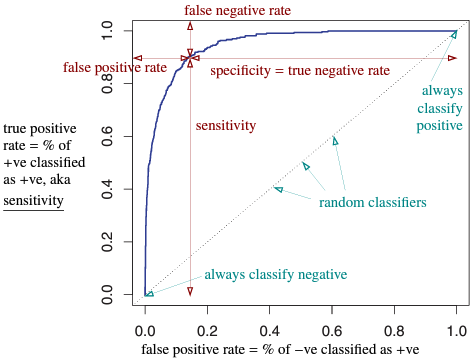
\includegraphics[scale=0.5]{./images/ROC-curve.png}
\end{multicols*}
\end{document}
